\noindent \textred{6.}
Given 
\[ 
    f_X(x) = \left\{
    \begin{aligned}
        &A \delta(x) &, x = 0 \\
        &e^{-1} (e^x + e^{-x}) &, 0 < x < 1 \\
        &0 &, \text{otherwise}
    \end{aligned}
    \right.
\]
\begin{enumerate}
    \item[(1)] Find $A$ so that $f_X(x)$ is a valid density. \\
    \myAnswer{
    $\int_{-\infty}^{\infty} f_X(x) dx = A + 1 - e^{-2} = 1 \Rightarrow \underline{A = e^{-2}}$.
    }
    \item[(2)] Write $f_X(x)$ in one line by using step functions. \\
    \myAnswer{
    $f_X(x) = \underline{e^{-2} \delta(x) + [u(x) - u(x-1)] \cdot e^{-1}(e^x + e^{-x})}$
    }
    \item[(3)] Sketch $f_X(x)$. \\
    \begin{figure}[!h]
        \centering
        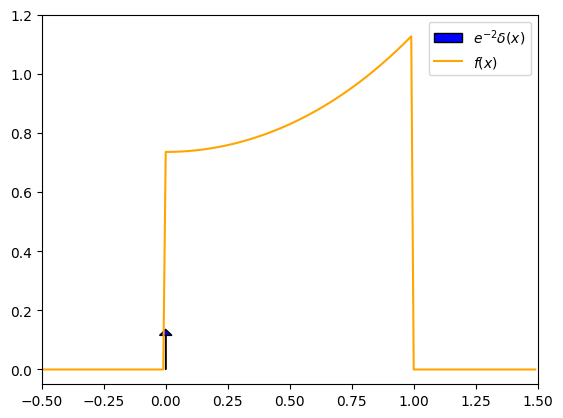
\includegraphics[width=0.5\linewidth]{HWs//HW2//figures/6-3.png}
    \end{figure}
    \item[(4)] Find $F_X(x)$ in analytical form. \\
    \myAnswer{
    \[
        F_X(x) = \left\{
            \begin{aligned}
            &0 &, x < 0 \\
            &e^{-2} + e^{-1}(e^x - e^{-x}) &, 0 \leq x < 1 \\
            &1 &, x \geq 1
        \end{aligned}
    \right.
    \]
    }
    \newpage
    \item[(5)] Sketch $F_X(x)$. \\
    \begin{figure}[!h]
        \centering
        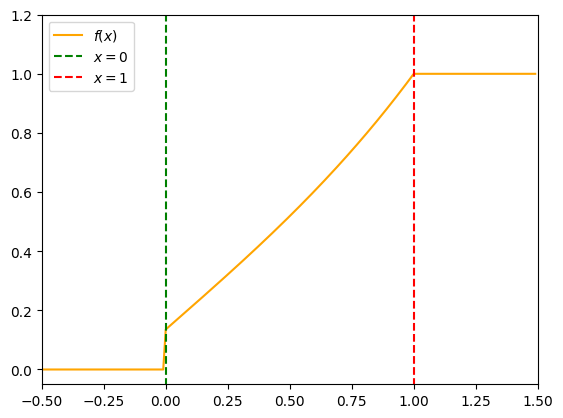
\includegraphics[width=0.5\linewidth]{HWs//HW2//figures/6-5.png}
    \end{figure}
\end{enumerate}